% Author: Magdalen Berns

\chapter{The Physiology of The Eye}

\label{anatomy} % For referencing

\lhead{\emph{The Anatomy of The Eye}}

\section{The Cornea and Lens}

The cornea is a transparent layer around 0.6mm thick, which curves over the
iris of the eye.\cite{yaylali1997corneal,thoft1983x,patel1994refractive}
With a mean refractive index of around 1.4 (about the same as water),
the cornea allows plenty of light to pass through. \Eref{eq:refractive}
shows Snell's Law of refraction for a light wave passing through two
different isotropic materials which have refractive indices $n_1$ and $n_2$,
respectively. The angle $\theta_1$ is normal to the boundary between $n_1$
and $n_2$ and the angle $\theta_2$ is normal to the boundary between $n_2$
and $n_1$.

\begin{equation}
n_1\sin\theta_1=n_2\sin\theta_2
\label{eq:refractive}
\end{equation}


The outermost surface of the cornea is made of epithelial cells which
are continually lost and replaced.\cite{jester1999cellular,hassell2010molecular}
The reproduction of cells is facilitated in part
by tear ducts, which  serve to moisten the eyes
and remove harmful bacteria.\cite{holly1977tear}

As people grow older, the radius of the cornea tends
to decrease and the cornea itself, takes on a more spherical shape.\cite{guirao2000optical}

There is a ciliary body of tissue which accommodates the cornea and secretes a fluid known as Aqueous Humour, which circles the circumference of the eye.\cite{}\fref{cilary_processes} shows some key ciliary processes at the region around the cornea.

\begin{figure}[htbp]
  \centering
    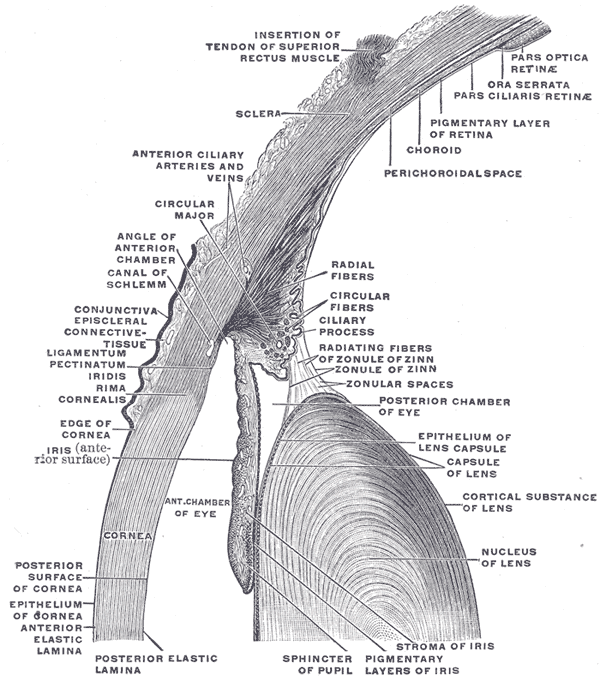
\includegraphics{figures/cilary_processes}
  \caption{Labelled sketch of ciary processes}
  \label{fig:cilary_processes}
\end{figure}

The lens of the eye refracts light which is being transmitted through it and it sits inside a bag of ciliary muscles which change the focal length of these
light waves. As humans age, these ciliary muscles weaken and this impairs the ciliary muscles' ability to accommodate the lens. The result of that is that the eye's ability to focus of visual imagery becomes impaired.\cite{} Taking eye exercise regularly, can help to prevent loss of ciliary muscle.

\section{Vitreous Humor}

\section{The Retina}
The retina is where light is changed from light waves into electrical signals
which we call brainwaves.

\section{Cones and Rods}

Cones and rods have photoreceptors which convert particular frequencies of
light waves into electrical signals so that the brain can interpret what
the eye has seen Whilst cones are not particularly sensitive to light,
they do aid to visual acuity because they grant us colour vision.\cite{}

A healthy and normal eye will pick up the full spectrum of colours. \ref{fig:wavelengths} shows normalised absorbency against wavelength for red, green and blue cones for an average human eye.

\begin{figure}[htbp]
  \centering
    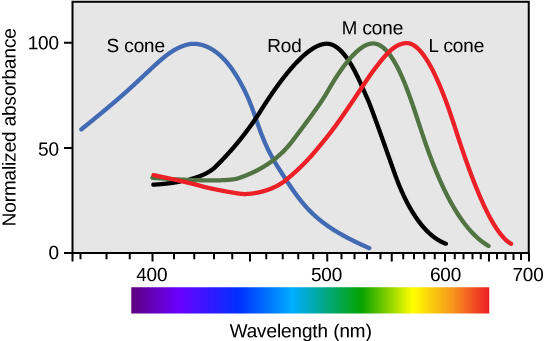
\includegraphics{figures/wavelengths}
  \caption{Normalised absorbency vs. wavelength, for an average eye.}
  \label{fig:wavelengths}
\end{figure}

If all the eye cones are not working then this can cause blindness to occur\cite{}

\section{The Optic Nerve}
